% !TEX root = ../thesis.tex
% !TEX spellcheck = en-US

%% Equations, tables and figures have their own numbering in Appendices
\renewcommand{\theequation}{B\arabic{equation}}
\setcounter{equation}{0}
\renewcommand{\thefigure}{B\arabic{figure}}
\setcounter{figure}{0}
\renewcommand{\thetable}{B\arabic{table}}
\setcounter{table}{0}


%% Appendices
\clearpage

\thesisappendix

% \section{Appendix \label{A}: Something something}
\section{Appendix}

\subsection{Source Files and Code}

\subsubsection*{A Tool for Crowd-Sourced Tagging of Chunked Job Ads}
\label{sub:A Tool for Crowd-Sourced Tagging of Chunked Job Ads}

The following repository contains the source code for the tool described in Section~\ref{subs:Supervised Multi-label Paragraph Classification}: \url{https://github.com/cle-ment/ma-thesis-crowdsource-text-tagger}
It was used to collect labels for paragraphs with the help of volunteers. To use it a server running \gls{MongoDB} and \gls{Node.js} is needed. A jupyer notebook for preprocessing data is provided in case other data shall be used.

\subsubsection*{Implementation of Final Experiments}
\label{sub:Implementation of Final Experiments}

This repository contains all source code needed to run the final experiments which are discussed in Section~\ref{sec:Experiments and Results}: \url{https://github.com/cle-ment/ma-thesis-experiments}
Unfortunately there was no time to make these completely reproducible from scratch as most experiments were run on \gls{AWS} instances with all needed libraries setup. The code can be also be run locally though if the python modules are installed and the code to set up the instances is provided if a similar setup is to be achieved.

\subsubsection*{\LaTeX\ Source of This Thesis}
\label{sub:This Thesis}

The source files for this document can be found in the following repository: \url{https://github.com/cle-ment/ma-thesis-tex}. The source files were made public for others to use them as a template and as a side-effect document the process of writing quite nicely:

\begin{figure}[h]
  \centering
  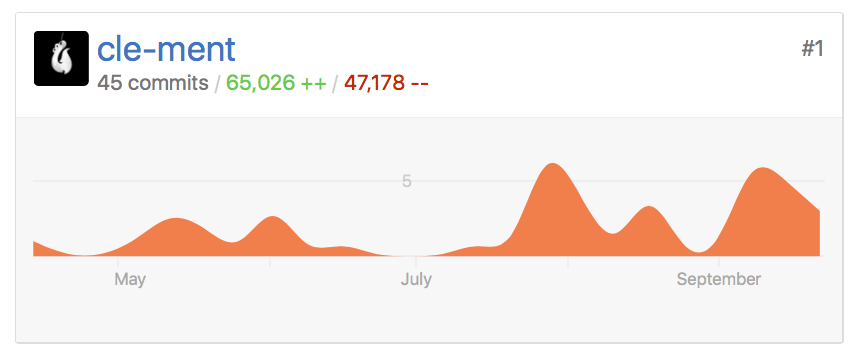
\includegraphics[width=0.7\textwidth]{img/git-tex.png}
  \caption{The activity on the thesis repository during the time of writing.}
\label{fig:git repo activity}
\end{figure}

\subsection{Google News Dataset and Word Embeddings}
\label{sub:Google News Dataset and Word Embeddings}

For constructing the Bag-Of-Means model explained in Section~\ref{subp:Bag-of-Means}, pre-computed word embeddings were used which were created by~\cite{Mikolov:2013ab} from a dataset from Google News. The dataset contains 300-dimensional vectors for 3 million words and phrases and can be obtained on the following website: \url{https://code.google.com/archive/p/word2vec/}

\clearpage
\subsection{Stopwords for N-grams}
\label{sub:Stopwords for N-grams}

This following list of English stop words is the one used in the \gls{scikit-learn} implementation for N-Grams and is taken from the \emph{Glasgow Information Retrieval Group}. The original list can be found at \url{http://ir.dcs.gla.ac.uk/resources/linguistic_utils/stop_words}.

\begin{minted}{html}

a, about, above, across, after, afterwards, again, against, all,
almost, alone, along, already, also, although, always, am, among,
amongst, amoungst, amount, an, and, another, any, anyhow, anyone,
anything, anyway, anywhere, are, around, as, at, back, be, became,
because, become, becomes, becoming, been, before, beforehand, behind,
being, below, beside, besides, between, beyond, bill, both, bottom,
but, by, call, can, cannot, cant, co, computer, con, could, couldnt,
cry, de, describe, detail, do, done, down, due, during, each, eg,
eight, either, eleven, else, elsewhere, empty, enough, etc, even,
ever, every, everyone, everything, everywhere, except, few, fifteen,
fify, fill, find, fire, first, five, for, former, formerly, forty,
found, four, from, front, full, further, get, give, go, had, has,
hasnt, have, he, hence, her, here, hereafter, hereby, herein,
hereupon, hers, herself, him, himself, his, how, however, hundred, i,
ie, if, in,inc, indeed, interest, into, is, it, its, itself, keep,
last, latter, latterly, least, less, ltd, made, many, may, me,
meanwhile, might, mill, mine, more, moreover, most, mostly, move,
much, must, my, myself, name, namely, neither, never, nevertheless,
next, nine, no, nobody, none, noone, nor, not, nothing, now, nowhere,
of, off, often, on, once, one, only, onto, or, other, others,
otherwise, our, ours, ourselves, out, over, own, part, per, perhaps,
please, put, rather, re, same, see, seem, seemed, seeming, seems,
serious, several, she, should, show, side, since, sincere, six,
sixty, so, some, somehow, someone, something, sometime, sometimes,
somewhere, still, such, system, take, ten, than, that, the, their,
them, themselves, then, thence, there, thereafter, thereby,
therefore, therein, thereupon, these, they, thick, thin, third, this,
those, though, three, through, throughout, thru, thus, to, together,
too, top, toward, towards, twelve, twenty, two, un, under, until, up,
upon, us, very, via, was, we, well, were, what, whatever, when,
whence, whenever, where, whereafter, whereas, whereby, wherein,
whereupon, wherever, whether, which, while, whither, who, whoever,
whole, whom, whose, why, will, with, within, without, would, yet,
you, your, yours, yourself, yourselves

\end{minted}

\clearpage

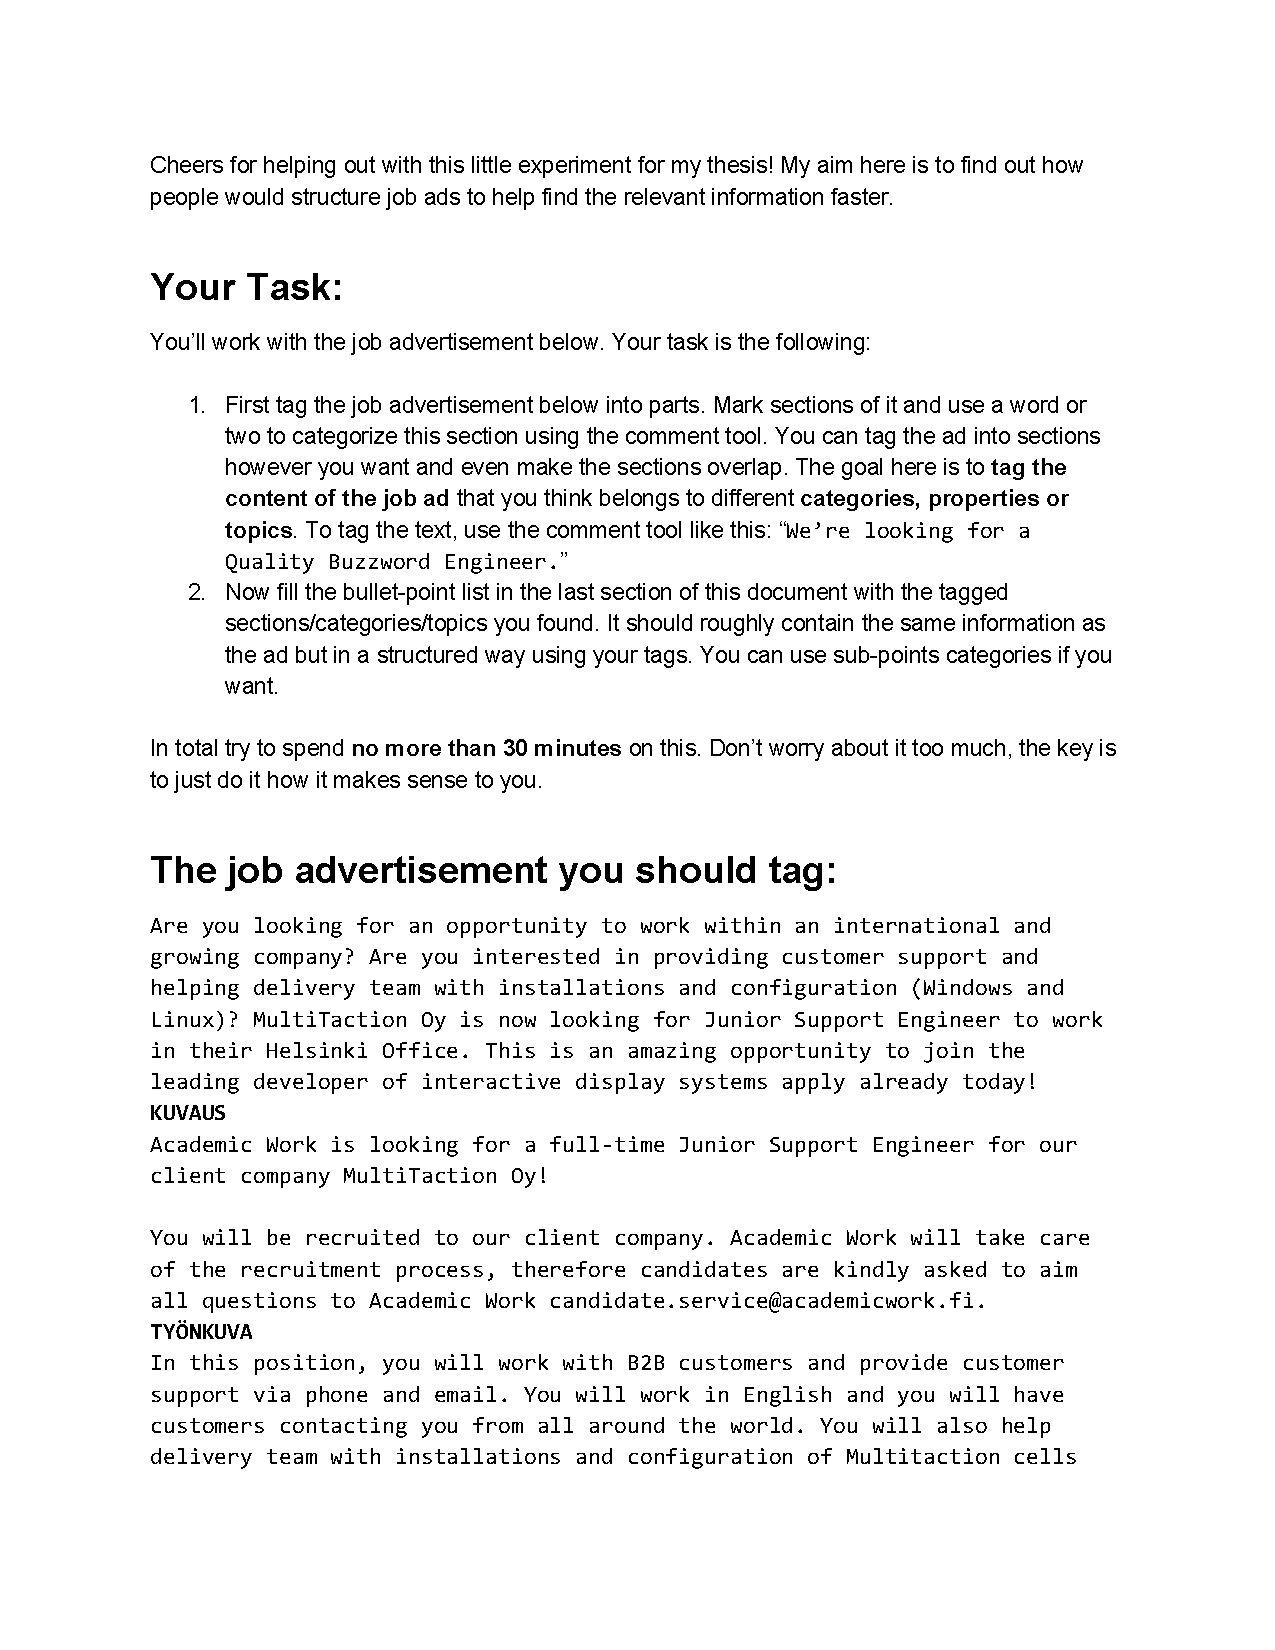
\includepdf[scale=0.71, pages=1, offset=85 -120, frame, pagecommand={
\subsection{Experiment Example: Inferring Structure of Job Advertisements}\label{sub:Understanding How Humans Structure Text}
This section shows an example of the task given to participants during the experiment described in Section~\ref{subs:Inferring Structure in Job Advertisements}. The task was presented in \gls{Google Docs}, enabling the participants to highlight and comment sections of the text.
}]{appendix/InferringStructureofJobAdvertisements-experiment-example.pdf}
\includepdf[scale=0.71, pages=2-, offset=85 -75, frame, pagecommand={}]{appendix/InferringStructureofJobAdvertisements-experiment-example.pdf}

\clearpage
\subsection{Collected Labels in Paragraph Experiment}
\label{sub:Collected Labels in Paragraph Experiment}

The following is the full collection of labels collected during the crowd-source paragraph labeling experiment described in Section~\ref{subs:Supervised Multi-label Paragraph Classification}:

\begin{minted}{json}
  {
      "Summary: Short introduction": [
          "intro", "job description", "job position", "description",
          "general", "job info", "general job description",
          "basic info", "job introduction ", "introduction",
          "general task", "general task ", "job",
          "job related field", "announcement", "announcement ",
          "about", "job description ", "overview",
          "position description", "job desription", "position",
          "kuvaus", "high level summary", "summary", "global work",
          "software integrations", "customer experience"

      ],
      "Person specification (Who you are)": [
          "required skill", "required skills", "capabilities",
          "skills", "skill", "requirements", "applicant's abilities",
          "actual requirements", "wished skills",
          "requirements ", "requirement", "competence",
          "skill requirement", "skill exception",
          "candidate's requirements", "prerequisite studies",
          "requirement ", "formal requirements", "job requirements",
          "important requirements", "job specific requirements",
          "common requirements", "start of skills list",
          "skills heading", "checklist for requirements ",
          "requirements title", "html5", "user-testing",
          "prototyping", "programming languages", "programming",
          "programming skills", "software development",
          "mobile development", "software developer",
          "language requirement", "languages", "langugage skills",
          "language requirements", "language", "language skill",
          "language skills", "web services integration", "software",
          "mgmt", "agile", "a360", "istqb", "bugtracking tool",
          "tools", "manollo", "clojure", "java", "scala", "design",
          "thread programming", "mobile", "spring", "angularjs",
          "additional skills", "bonus skills", "desired skill",
          "applicant's personality", "personal", "soft skills",
          "personal skill", "social skills", "characteristics",
          "habits", "character", "attitude", "transaction management",
          "technical skills", "domain skill", "project management",
          "quality assurance", "analysis", "tracking", "testing",
          "communication skill", "travel requirements",
          "traveling requirements", "travel", "expected values",
          "time commitment", "time", "company's needs", "performance",
          "employee qualities ", "degree", "job specific tag",
          "knwoledge", "education", "knowledge", "capability",
          "expectations", "background", "job challenge",
          "business-minded", "qualifications", "asset",
          "working hours", "detailed info", "innovation",
          "tech", "experience requirement", "experience",
          "integration experience", "previous experience",
          "work experience", "full time", "temps", "job form",
          "job classification ", "extent", "position type",
          "job duration ", "job type", "employment type", "work type"

      ],
      "Benefits (What we give)": [
          "marketing the job", "goal", "selling the job",
          "marketing of the company", "sales pitch", "remuneration",
          "motivation", "self-advertising", "benefits", "reward",
          "treats", "job benefits", "company's treats",
          "opportunities", "additional job opportunities",
          "incentive", "additional opportunity", "salary", "offering",
          "we offer", "job offer", "compensation", "oppoturnity",
          "what you get", "offer"
      ],
      "Job specification (What you give)": [
          "job title ", "seniormanager", "clinicalcontractcoordinator",
          "search", "ask", "what", "work title", "need", "looking for",
          "title", "job title" "functions", "responsibilities heading",
          "role", "job role", "detailed task", "about the role",
          "duties", "checklist for job description ", "general tasks",
          "job responsibilities", "work summary", "task titles",
          "responsibilites", "main tasks", "tasks", "responsibility",
          "responsibilities", "task", "team", "unit",
          "unit description", "team title", "company branch", "level",
          "asw", "practicalities", "position level", "department",
          "organisational position", "unit of the company",
          "unit of company", "company unit descriptions",
          "location of job", "finlandjob", "location ", "job location",
          "where", "location data", "sijainti", "paikka", "place",
          "office", "job ad", "location", "finland", "duration",
          "time frame", "dates", "starting date", "time period",
          "conditions"
      ],
      "Company (Who we are)": [
          "manpower", "bayer", "bayer2013", "bayerr&d",
          "bayerrecruiting ", "kemira", "reaktor", "company name",
          "tieto", "paf", "company", "company info",
          "introduction to organization", "company description",
          "company ", "employer`s information", "general company info",
          "history of employer", "company description ",
          "company facts", "organisatio", "employer info",
          "employer description", "website of employer",
          "website contact info", "website", "employer listing ",
          "service offering", "product line",
          "detailed information on productline",
          "company introduction", "intro to company", "who",
          "company presentation", "organization", "ccompany details",
          "company details", "organisation description", "about us",
          "company data", "industry", "field of operations", "retail",
          "business type", "consulting", "employer", "money games",
          "non-discrimination", "equal opportunity", "company vision",
          "company culture", "company policy"
      ],
      "Next steps": [
          "applying", "contract", "selection", "apply", "how to apply",
          "apply info", "application process",
          "application information", "application practicalities ",
          "practical information", "application instructions",
          "how to apply?", "instructions", "application submission",
          "application", "application procedure", "attachments",
          "application details", "opening date", "closing date",
          "deadline ", "deadline for application", "dealine",
          "application deadline", "deadline", "timetable",
          "auxiliary target group", "encouragement", "invitation ",
          "invitation" "employer listing", "more about position",
          "further info", "further information", "more information",
          "futrher information", "lisätieto", "more info",
          "additional information", "link", "contact details",
          "contact person", "contact info", "contact",
          "contact practicalities ", "contact person name ",
          "contact person title ", "contact person mail ",
          "job contact information", "job inquiry email",
          "phone number", "contacts", "contact ddetails",
          "help", "signature ", "contact ", "contact person title",
          "details", "contact information", "recruiter", "recruiting",
          "contact agent", "job agent", "about job agent ",
          "about job agent"
      ],
      "Other": [
          "empy", "-", "empty", "none", "nothing", "empty space",
          "no data", "start of list", "heading", "section title",
          "header", "introductory phrase ", "transition", "subheader",
          "headline", "question", "job id", "number", "job number",
          "keywords", "90% bullshit", "blabla",
          "signal for interview question", "bullshit", "useless info",
          "crap", "information", "info"
      ]
  }
\end{minted}
